\subsection{Measurement Errors and their Effect on the Parameter Recovery} \label{sec:results_errors}

\Wilma{[TO DO: Comment from HW: This Section has three parts:}
\\\Wilma{-- convergence of the integral}
\\\Wilma{-- testing the approximation}
\\\Wilma{-- underestimating errors}
\\\Wilma{It seems to me that the basic Section:
What is the impact of the errors? Is missing. That should be the center piece, and the other three aspects should be quick summary notes, only 1-2 sentences long.]} \Wilma{[I'll try to address this with a plot mean(SE) vs. proper motion error - also for cold population (currently running on wolf).]}

\paragraph{Convergence of the error integral.} \Wilma{[TO DO: Move this section and plot to theory part.]} In Section \ref{sec:likelihood} we introduced how we convolve the model probability with the measurement errors. In the absence of distance errors, the accuracy of the parameter recovery is limited by insufficient sampling of the MC convolution integral in Equation \ref{eq:errorconv}. Test \ref{test:isoSphFlexErrConv_MC_vs_error} in Table \ref{tbl:tests} and Figure \ref{fig:isoSphFlexErrConv_MC_vs_error} investigate how many MC samples are needed, given the size of the velocity error, for the integral to be accurate within certain limits: For each $\delta \mu \in [2,3,4,5] \text{ mas yr}^{-1}$ we set up $N_\text{mock} = 4$ mock data sets and evaluate the likelihood for different $N_\text{error}$. We used $N_\text{conv} =$ 800 and 1200 MC samples to calculate the numerically converged likelihood for proper motion errors $\delta \mu \leq 3 \text{mas yr}^{-1}$ and $\delta \mu > 3 \text{mas yr}^{-1}$, respectively (see left panels in Figure \ref{fig:isoSphFlexErrConv_bias_vs_SE}). We determined the bias 
\begin{equation*}
\text{BIAS}(N_\text{error},\delta \mu) \equiv \frac{1}{N_\text{mock}} \sum_{j=1}^{N_\text{mock}} \left[ \langle p_i \rangle (N_\text{error},\delta \mu)\right]_j - \left[ \langle p_i \rangle (N_\text{conv},\delta \mu)\right]_j,
\end{equation*}
where $\left[ \langle p_i \rangle (N_\text{error},\delta \mu)\right]_j$ is the best estimate for the $i$-th model parameter $p_i \in \pmodel$ from the analysis of the $j$-th mock data realisation with $\delta \mu$ using $N_\text{error}$ MC samples. From this we then generated the curves $N_{\text{error},i} (\delta v_\text{max},\text{BIAS})$ in Figure \ref{fig:isoSphFlexErrConv_MC_vs_error} by linear interplolation, that show how many MC samples are needed for parameter $p_i$ given a velocity error and a systematic bias in units of the standard error (SE) of the estimate. The proper motion error $\delta \mu$ translates to heteroscedastic \Wilma{[TO DO: make sure that this word is written correctly everywhere.]} velocity errors according to
\begin{equation}
\delta v [\text{km s}^{-1}] \equiv 4.74047 \cdot r[\text{kpc}] \cdot \delta \mu [\text{mas yr}^{-1}], \label{eq:vmax}
\end{equation}
where $r$ is the distance of the star to the sun. The largest velocity error $\delta v_\text{max}$ within the sample is at $r_\text{max}$. We find in Figure \ref{fig:isoSphFlexErrConv_MC_vs_error} the relation
\begin{equation*}
N_{\text{error},i} (\delta v_\text{max},\text{BIAS}) \propto \left( \delta v_\text{max} \right)^2.
\end{equation*}
Figure \ref{fig:isoSphFlexErrConv_MC_vs_error} also demonstrates that different model parameters do not have the same sensitivity to the numerical inaccuracies introduced by insufficient sampling. \Wilma{[TO DO: Comment from Jo: I think it is important to test, if the MC vs error plot depends on number pf stars. Maybe test it with less stars (5000), to test this quickly. Naively, I would expect a large depedence on Ndata.]}

\paragraph{Testing the error convolved likelihood approximation.} \Wilma{[TO DO: Comment from HW: This is a very technical aspect: it should be summarized in 1-2 sentences; you neither have to provide code documentation, nor document effort. The reader wants the upshot.]} \Wilma{[TO DO: Jo doesn't like subsub(sub?)sections... Remove.]} In absence of distance (modulus) errors our approximation for the likelihood, which is the model probability convolved with the measurement uncertainties in Equation \ref{eq:errorconv}, is equal to the true likelihood. In case there \emph{are} distance modulus errors, this likelihood links the range of possible velocities (specified by the measurement errors in line-of-sight velocity, proper motion and distance modulus) to a fixed but slightly wrong position, as we ignore the distance error in the position. As the link between position and velocity provides the information about the potential, this will lead to systematic biases in the parameter recovery the larger the distance error becomes. In Test \ref{test:isoSphFlexErrConv_bias_vs_SE} in Table \ref{tbl:tests} and Figure \ref{fig:isoSphFlexErrConv_bias_vs_SE} we investigate the capabilities of Equation \ref{eq:errorconv} with and without distance modulus errors.
\\The left column of panels in Figure \ref{fig:isoSphFlexErrConv_bias_vs_SE} shows how well the approximation works in the absence of distance errors. There seemed to be no biases in the parameter recovery, independent of the size of the proper motion error. Overall the standard errors on the recovered parameters are quite small (a few percent at most for 10,000 stars), which demonstrates that, if we perfectly knew the measurement errors, we still could get very precise constraints on the potential. The constraints also get tighter the smaller the proper motion error becomes. We found that for $\delta \mu = 1 \text{ mas yr}^{-1}$ the precision of the recovered parameters reduce by $\sim$ half compared to $\delta \mu = 5 \text{ mas yr}^{-1}$. \Wilma{[TO DO: Comment from HW: This seems to be a (sensible) statement about the impact of the errors. Why is it under the heading of testing an approximation?]}
\\The right column of panels in Figure \ref{fig:isoSphFlexErrConv_bias_vs_SE} demonstrates the failure of our adopted likelihood approximation in the case of large distance modulus errors. The larger the $\delta(m-M)$, the wronger the recovered parameters become: The systematic biases can get many SEs large. We find however that in case of $\delta(m-M) \leq 0.2 \text{ mag}$ (if also $\delta \mu \leq 2 \text{ mas yr}^{-1}$ and a maximum distance of $r_\text{max} = 3 \text{ kpc}$, see Test \ref{test:isoSphFlexErrConv_bias_vs_SE} in Table \ref{tbl:tests}) the parameters can still be recovered within 2 SEs. For most model parameters (except $\ln(\sigma_{z,0} / 200\text{ km s}^{-1})$, as shown in the figure, and $\ln(h_R/ 8\text{ kpc})$) even $\delta(m-M) \leq 0.3 \text{ mag}$ still gives biases smaller than 2 SEs. This corresponds to a relative distance error of $\sim10\%$. This encourages us that for smaller distance modulus errors we really could use our likelihood approximation in Equation \ref{eq:errorconv}, which is computationally cheaper than a proper treatment, also on real data sets.\\

We found that in case we perfectly knew the measurement errors (and the distance error is negligible), the convolution of the model probability with the measurement errors gives precise and accurate constraints on the model parameters - even if the error itself is quite large. \Wilma{[TO DO: That statement should be the last, concluding sentence of one of the previous sections. Then its fresh in the reader's mind, and does not need repeating.]}



\paragraph{Underestimation of the proper motion error.}  Now we investigate what would happen if the quoted measurement errors, e.g. the proper motion errors, were actually smaller than the true errors. Figure \ref{fig:isoSphFlexErrSyst} shows the case for two different stellar populations and an error underestimation of 10\% and 50\%. 
\\Overall the parameter recovery gets worse the larger the proper motion error and the stronger the underestimation. The relation between the bias due to error misjudgment and the size of the proper motion error seems to be linear.
\\For the recovery of the isochrone potential scale length $b$ the hotness of the population does not matter (see lower left panel in Figure \ref{fig:isoSphFlexErrSyst}). The circular velocity $v_\text{circ}(R_\odot)$ is, as always, better measured by cooler than by hotter populations (see upper left panel in Figure \ref{fig:isoSphFlexErrSyst}). 
\\We find that the recovery of the qDF parameters on the other hand is more strongly affected by the misjudgment of the velocity error for \emph{cooler} stellar popluations. The measured velocity dispersion is the convolution of the intrinsic dispersion with the measurement errors. If the proper motion error is underestimated, the deconvolved velocity dispersion is larger than the intrinsic velocity dispersion and the relative difference is bigger for a cooler population (see upper right panel for $\sigma_{z,0}$ in Figure \ref{fig:isoSphFlexErrSyst}). The intrinsic velocity dispersion is also cooler at larger radii than at smaller radii, therefore the deconvolved dispersion is overestimated more strongly at large $R$ and the velocity dispersion scale length will be overestimated as well (see lower left panel for $h_{\sigma,z}$ in Figure \ref{fig:isoSphFlexErrSyst}). We get analogous results for the qDF parameters $\sigma_{R,0}$ and $h_{\sigma,R}$. The recovery of the tracer density scale length $h_R$ is not affected by the misjudgment of velocity errors. 
\\The most important and encouraging result from Figure \ref{fig:isoSphFlexErrSyst} is, that for an underestimation of $10\%$ the bias is still $\lesssim 2$ sigma for 10,000 stars \Wilma{[TO DO: Check]} - even for proper motion errors of almost $3$ mas/yr.

%=============================================================

\begin{figure*}
\centering     %%% not \center
\subfigure[$N_* = 10,000$]{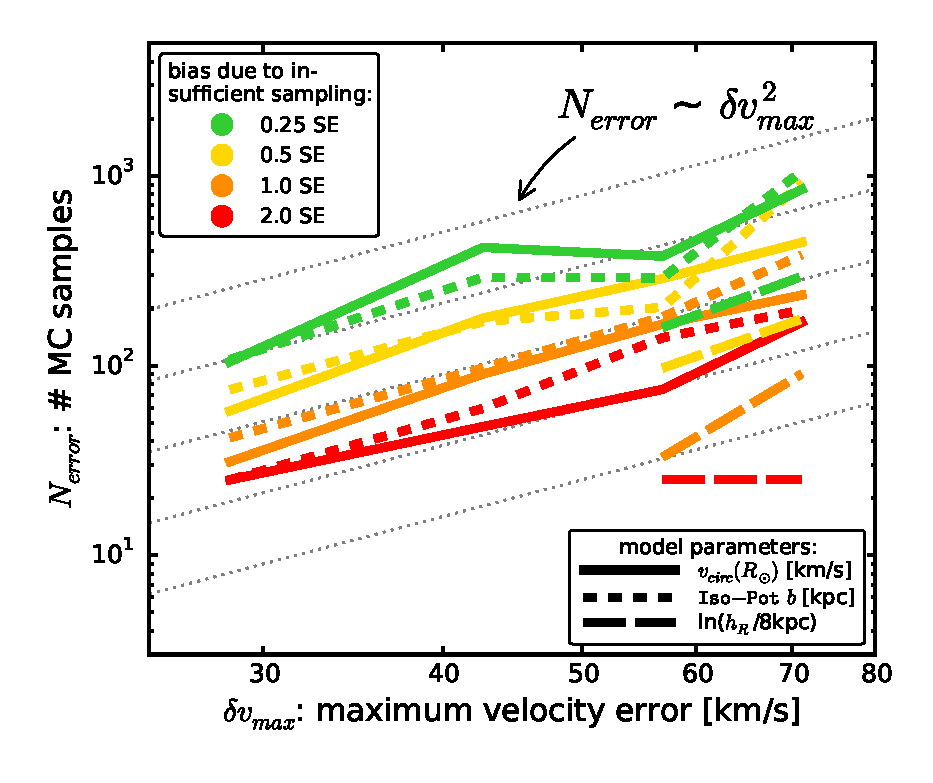
\includegraphics[width=60mm]{figs/isoSphFlexErrConv_MC_vs_error_2.eps}}
\subfigure[$N_* = 5,000$]{
\includegraphics[width=60mm]{figs/Coming-Soon-Placeholder.eps}}
\caption{Number of Monte Carlo (MC) samples $N_\text{error}$ needed for the numerical error convolution in Equation \ref{eq:errorconv}, given the maximum velocity error $\delta v_\text{max}$ in the sample to reach a given accuracy.  An insufficient sampling of the convolution integral leads to systematic biases in the reconstruction of the true model parameters. The size of the bias is color coded as indicated in the legend and is given in units of the standard error (SE).  The model parameters, marked by different symbols, have different sensitivities to the numerical inaccuracy of the error convolution, therefore the range in $N_\text{error}$ for the same given bias. Here we assume that the distance error is zero and the proper motion error $\delta \mu$ translates to a velocity error according to Equation \ref{eq:vmax} and $\delta v_\text{los} \ll \delta v_\text{max}$. All model parameters are listed in Table \ref{tbl:tests} as Test \ref{test:isoSphFlexErrConv_MC_vs_error}. The number of MC samples needed increases with the velocity error as $N_\text{error} \propto \left( \delta v_\text{max} \right)^2$, as can be seen especially well in the inset figure for the potential parameter $v_\text{circ}(R_\odot)$. All lines are fits of this functional form to each four points derived for a given model parameter (symbol) and bias (color). The large scatter in the points comes from low number statistics and errors introduced by linear interpolation of the bias vs. $N_\text{error}$ relation found from the analyses. \Wilma{[TO DO: rename $h_{\sigma R}$ to $h_{\sigma,R}$, $\sigma_R$ to $\sigma_{R,0}$ and analogous for $z$] [TO DO: some of the 25 MC sample analyses have to be re-done. (Currently running on cluster.)] [TO DO: Rewrite caption. I changed the whole plot.] [TO DO: Replace right plot with new plot with $N_* = 5,000$] [TO DO: Use $N_*$ everywhere where applicable] [TO DO: Intriduce $N_*$ somewhere.]}}
\label{fig:isoSphFlexErrConv_MC_vs_error}
\end{figure*}


%=============================================================

\begin{figure}
\plotone{figs/isoSphFlexErrConv_bias_vs_SE.eps}
\caption{Parameter recovery using the approximation for the measurement error convolved likelihood in Equation \ref{eq:errorconv}. All model parameters used to create the mock data sets analyzed for this figure are given as Test \ref{test:isoSphFlexErrConv_bias_vs_SE} in Table \ref{tbl:tests}. The mock data sets in the left panels have only errors in line-of-sight velocity and proper motions, while the data sets in the right panels also have distance modulus errors, as indicated in the legends in the first row. The size of the error is color coded. The other panels plot the offset of the recovered model parameter to the true parameter vs. the relative standard error for two of the seven model parameters, the potential parameter $v_\text{circ}(R_\odot)$ and qDF parameter $\sigma_{z,0}$. For data sets with proper motion error errors $\delta(m-M) \leq 3 \ \text{mas yr}^{-1}$ Equation \ref{eq:errorconv} was evaluated with $N_\text{error}=800$, for $\delta(m-M) > 3 \ \text{mas yr}^{-1}$ we used $N_\text{error}=1200$. In the absence of distance errors Equation \ref{eq:errorconv} gives unbiased results. For $\delta(m-M) \geq 3 \text{mas yr}^{-1}$ (which corresponds in this test to $\delta v_\text{max} \lesssim 43 \ \text{km s}^{-1}$, see Equation \ref{eq:vmax}) however biases of several sigma are introduced as Equation \ref{eq:errorconv} is only an approximation for the true likelihood in this case. \Wilma{[TO DO: rename  $\sigma_z$ to $\sigma_{z,0}$] [TO DO: Show b instead of $\sigma_z$ and don't comment the small offset.] [TO DO: Incorporate legends within the bottom panels, with only one point (numpoints=1)] [TO DO: Use viridis color map] [TO DO: Add the additional analyses I did in the left column, e and f.]}}
\label{fig:isoSphFlexErrConv_bias_vs_SE}
\end{figure}

%=============================================================

\begin{figure}
\plotone{figs/Coming-Soon-Placeholder.eps}
\caption{\Wilma{[TO DO: This should be a figure that plots precision (SE) vs. proper motion error for a hot and a cool population (for no distance error). This is to demonstrate the effect of measurement errors in general.]}}
\label{fig:???}
\end{figure}



%=============================================================

\begin{figure}
\plotone{figs/isoSphFlexErrSyst_offset_vs_error.eps}
\caption{Effect of a systematic underestimation of proper motion errors in the recovery of the model parameters. The true model parameters used to create the mock data are summarized as Test \ref{test:isoSphFlexErrSyst} in Table \ref{tbl:tests}, four of them are given on the $y$-axes and the true values are indicated as black dashed lines. The velocities of the mock data were perturbed according to Gaussian errors in the RA and DEC proper motions as indicated on the $x$-axis. The circles and triangles are the best fit parameters of several mock data sets assuming the proper motion uncertainty, with which the model probability was convolved, was underestimated in the analysis by 10\% or 50\%, respectively. The error bars correspond to 1 sigma confidence. The lines connect the mean of each two data realisations and are just to guide the eye. \Wilma{[TO DO: rename $h_{\sigma z}$ to $h_{\sigma,z}$, $\sigma_z$ to $\sigma_{z,0}$] [TO DO: Potential and/or population names in typewriter font]}}
\label{fig:isoSphFlexErrSyst}
\end{figure}

%=============================================================

\Wilma{[TO DO: Comment from Jo: Always use 'uncertainty' when describing how ou deal with the errors. 'Error' means the actual error (difference between observed and true).]}
